\phantomsection\numberedsection{RF2 Gestión general de Productos (\textit{Listado})}

\subsection*{Descripción}
El sistema muestra una lista de productos en formato \textit{DataGrid} en la sección de productos. La lista incluye los atributos de cada producto que permiten identificarlo, tanto los atributos de sistema: Thumbnail, SKU y label, como los atributos personalizados por el usuario, con una limitación de la descripción de 50 caracteres. Además, la interfaz permite buscar productos por SKU, y por label, y proporciona botones para editar, añadir y borrar productos, aunque la funcionalidad de estos botones se detalla en otros casos de uso.

\vspace{0.15cm}

\textbf{Pre-condición}\par
El usuario ha iniciado sesión en Mini PIM y tiene acceso a la sección de productos.\par
\vspace{0.15cm}

\textbf{Post-condición}
\begin{itemize}
    \item Caso de éxito: El sistema muestra la lista de productos con todos los atributos visibles en un \textit{DataGrid}.
    \item Caso de error: El sistema muestra un mensaje indicando que no hay productos disponibles para mostrar.
\end{itemize}

\textbf{Prioridad: }
Alta
\vspace{0.15cm}

\textbf{Autor: }
Diego Sicre\par
\vspace{0.15cm}

\textbf{Control de cambios: } Versión 1: Definición del caso de uso

\numberedsubsection{Escenario principal}
\begin{enumerate}
    \item El usuario selecciona la opción \enquote{Productos} desde el menú principal.
    \item El sistema carga y muestra un \textit{DataGrid} con la lista de productos disponibles.
    \item Cada fila en el \textit{DataGrid} incluye los siguientes datos:
    \begin{itemize}
        \item Thumbnail (imagen en miniatura del producto)
        \item SKU (atributo de sistema)
        \item Label (etiqueta del producto)
        \item Atributos personalizados (hasta 5 atributos de usuario)
    \end{itemize}
    \item El sistema permite al usuario buscar productos mediante los campos SKU o label.
    \item El usuario ingresa un SKU en el campo de búsqueda y confirma la acción.
    \item El sistema filtra la lista de productos para mostrar solo aquellos que coinciden con el SKU o label ingresado.
    \item Para cada fila del \textit{DataGrid}, el sistema permite seleccionar y realizar la acción de Editar, Añadir y Borrar.
\end{enumerate}

\numberedsubsection{Escenarios alternativos}
\begin{description}
    \item[3.a] El sistema no encuentra productos que coincidan con la búsqueda por SKU o label.
    \begin{enumerate}
        \item[3.a.1] El sistema muestra un mensaje indicando que no hay productos que coincidan con los criterios de búsqueda.
    \end{enumerate}

    \item[*.a] El usuario cancela la búsqueda sin ingresar un SKU o un label.
    \begin{enumerate}
        \item[*.a.1] El sistema muestra la lista completa de productos sin aplicar filtros.
    \end{enumerate}

    \item[5.a] No hay productos registrados en el sistema.
    \begin{enumerate}
        \item[5.a.1] El sistema muestra un mensaje indicando que no hay productos disponibles para mostrar.
    \end{enumerate}
\end{description}

\numberedsubsection{Casos de Prueba}
\underline{Escenario: Principal}\par
\vspace{0.15cm}
\textbf{Dado} que el usuario ha iniciado sesión en su cuenta en Mini PIM,\par
\textbf{Cuando} selecciona la opción de \enquote{Productos} en el menú principal,\par
\textbf{Entonces} el sistema carga y muestra la lista de productos en un \textit{DataGrid} con todos los atributos visibles.\par
\vspace{0.20cm}

\underline{Escenario: Alternativo 3.a}\par
\vspace{0.15cm}
\textbf{Dado} que el usuario intenta buscar un producto mediante SKU o label,\par
\textbf{Cuando} no hay productos que coincidan con los criterios de búsqueda,\par
\textbf{Entonces} el sistema muestra un mensaje indicando que no hay productos que coincidan.\par
\vspace{0.20cm}

\underline{Escenario: Alternativo *.a}\par
\vspace{0.15cm}
\textbf{Dado} que el usuario ha abierto la sección de productos,\par
\textbf{Cuando} cancela la búsqueda sin ingresar un SKU o label,\par
\textbf{Entonces} el sistema muestra la lista completa de productos sin aplicar filtros.\par
\vspace{0.20cm}

\underline{Escenario: Alternativo 5.a}\par
\vspace{0.15cm}
\textbf{Dado} que el usuario ha iniciado sesión en Mini PIM,\par
\textbf{Cuando} selecciona la opción de \enquote{Productos} y no hay productos registrados en el sistema,\par
\textbf{Entonces} el sistema muestra un mensaje indicando que no hay productos disponibles para mostrar.\par
\vspace{0.20cm}


\numberedsubsection{Bocetos}
\begin{figure}[H]
    \includegraphics[width=1\linewidth]{mockups/RF2- Gestión General de Productos (listado).png}
    \caption{Listado de Productos}
   \end{figure}
\vspace{1.0cm}

\begin{figure}[H]
    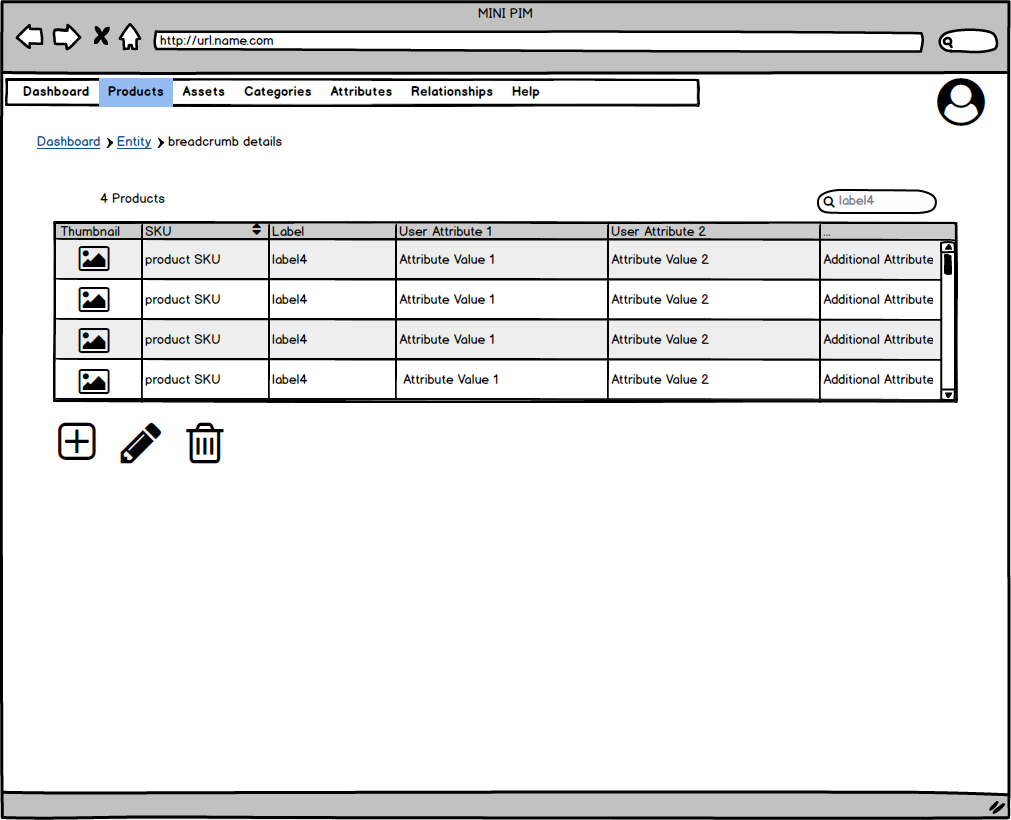
\includegraphics[width=1\linewidth]{mockups/RF2- Gestión General de Productos (listado por búsqueda).png}
    \caption{Listado de Productos con búsqueda filtrada por label}
   \end{figure}
\vspace{1.0cm}

\newpage %Inicia en una nueva página otro caso de uso